\begin{figure}[t!]
\begin{tabular}{@{\hskip 2mm}c@{}c@{}}
\begin{subfigure}[b]{0.5\textwidth}
\begin{center}
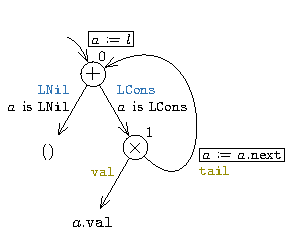
\includegraphics[scale=1.35]{chapters/figures/figValueTreeVarList.pdf}
\end{center}
\vspace{4px}
\caption{\label{fig:valuetreevar}$\mathcal{V}(l)$}
\end{subfigure}%
&
\begin{subfigure}[b]{0.5\textwidth}
\begin{center}
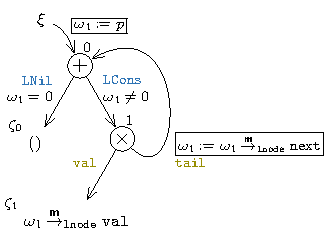
\includegraphics[scale=1.35]{chapters/figures/figValueTreeClist.pdf}
\end{center}
\caption{\label{fig:valuetreelifted}$\mathcal{V}(\lifted{list}{\mem{}}{lnode}{p})$}
\end{subfigure}%
\\
\end{tabular}
\caption{\label{fig:valuetreeapproxeg}Value trees for a \type{List} variable $l$ and a lifted expression \lifted{list}{\mem{}}{lnode}{p} respectively.}
\end{figure}